\documentclass[11pt]{beamer}
\usepackage[english]{babel}    % faire du français
\usepackage[T1]{fontenc}        % accents dans le DVI
\usepackage[utf8]{inputenc}   % accents dans le source
\usepackage{graphicx}
\usepackage{amssymb}
\usepackage{mathtools}
\usepackage{color, colortbl}

\usepackage{libertine}
\renewcommand*\familydefault{\sfdefault}  %% Only if the base font of the document is to be sans serif

\setbeamersize{text margin left=10pt,text margin right=10pt}
\setbeamertemplate{navigation symbols}{}

\pgfdeclareimage[height=\textheight,width=\textwidth]{bkg}{frontAgaetis}
\setbeamertemplate{background}{\pgfuseimage{bkg}}

\setbeamercolor{frametitle}{fg=orange}
\setbeamercolor{itemize item}{fg=orange}
\setbeamertemplate{itemize item}[circle]
\setbeamercolor{itemize subitem}{fg=orange}
\setbeamertemplate{itemize subitem}[triangle]
\setbeamercolor{enumerate item}{fg=orange}
\setbeamercolor{enumerate subitem}{fg=orange}

\usefonttheme[onlymath]{serif}

\definecolor{paleOrange}{RGB}{255,204,153}
\definecolor{forestGreen}{RGB}{0,204,0}
\definecolor{veryPaleOrange}{RGB}{255,229,204}
\setbeamertemplate{blocks}[rounded][shadow=true]
\beamerboxesdeclarecolorscheme{suppervise}{orange}{paleOrange}

\newcommand{\tabitem}{~~\llap{\textbullet}~~}

\author{\textcolor{black}{Introduction à l'apprentissage automatique} \hfill \textcolor{orange}{Léo Beaucourt} \hfill \textcolor{black}{Agaetis}}
\setbeamertemplate{footline}
{                  
  \leavevmode%
  \hbox{\begin{beamercolorbox}[wd=.85\paperwidth,ht=2.5ex,dp=1.125ex,leftskip=.3cm plus1fill,rightskip=.3cm]{author in head/foot}%
      \insertauthor
  \end{beamercolorbox}}%
  \hbox{\begin{beamercolorbox}[wd=.05\paperwidth,ht=2.5ex,dp=1.125ex,leftskip=.3cm plus1fill,rightskip=.3cm]{author in head/foot}%
      \textcolor{orange}{\insertframenumber/\inserttotalframenumber}
  \end{beamercolorbox}}%
  \vskip0pt%
}

\begin{document}

\begin{frame}

  \vspace{5cm}
  \begin{center}
    \Large
    \textcolor{orange}{Introduction à l'apprentissage automatique:}\\
    \textcolor{orange}{La régression linéaire}\\
    \normalsize
    \vspace{0.5cm}
    Léo Beaucourt
  \end{center}
    
\end{frame}

\setbeamertemplate{background}{}


\begin{frame}{Pourquoi la régression linéaire?}

  \begin{itemize}
  \item La régression linéaire: le \textcolor{orange}{``\textit{Hello world!}''} du \textit{ML}
    \vspace{0.2cm}
  \item Résolution d'un problème de Data science: \textit{Prédiction d'un prix}
    \vspace{0.2cm}
  \item En pratique: \textit{Python}, \textit{Jupyter}. Packages \textit{numpy} \textit{pandas} et \textit{matplotlib}.
    \vspace{0.2cm}
  \item Pas de (trop) de math ...
  \end{itemize}

  \vfill
  \begin{center}
    \large
    \textcolor{orange}{Allez, on démarre en douceur ...}
  \end{center}

\end{frame}

\begin{frame}{\underline{\href{https://www.youtube.com/watch?v=O52jAYa4Pm8}{\textit{Psycho killer}}}, qu'est ce que c'est?}
  \begin{figure}
    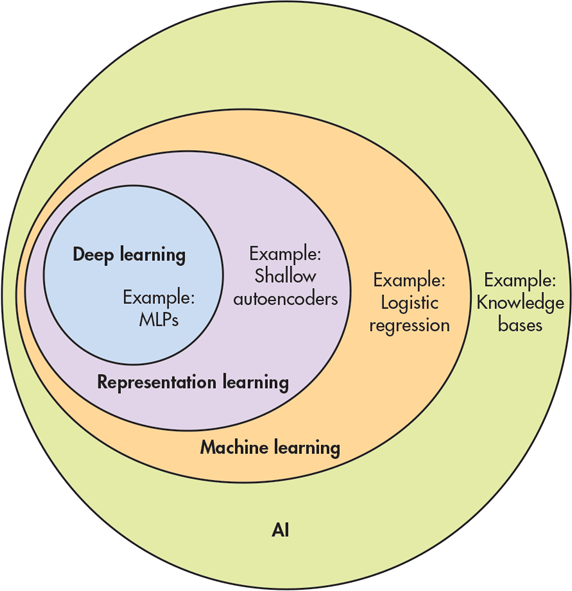
\includegraphics[width=0.6\textwidth]{figs/aiVennDiagram.png}
  \end{figure}
  \tiny
  \vspace{-1cm}
  \textit{[From \href{http://www.deeplearningbook.org/}{\color{blue}{MIT Press book Deep Learning}}]}
\end{frame}


\begin{frame}{Le \textit{Machine Learning}, qu'est ce que c'est?}

  \begin{itemize}
  \item \textbf{Arthur Samuel:}
    \begin{itemize}
      \normalsize
    \item \textit{The field of study that gives computers the ability to learn without being explicitly programmed.}
    \end{itemize}
    \vspace{0.2cm}
  \item \textbf{Tom Mitchell:}
    \begin{itemize}
      \normalsize
    \item \textit{A computer program is said to learn from experience E with respect to some class of tasks T and performance measure P, if its performance at tasks in T, as measured by P, improves with experience E.}
    \end{itemize}
    \vspace{0.5cm}
  \item \textbf{\textcolor{orange}{L'idée: }} Une machine apprend \textit{seule} à réaliser une tache complexe à l'aide de processus itératifs simple.
  \end{itemize}
  
\end{frame}

\begin{frame}{Les principaux types d'apprentissage}
  \hspace{0.25\textwidth}
  \begin{beamerboxesrounded}[scheme=suppervise,width=0.5\textwidth]{\textcolor{black}{Supervisé}}
    \begin{itemize}
      \tiny
    \item Utilise des données \textit{labélisées}
    \item La machine apprend par l'exemple
    \item \textit{Prédis} le résultat pour de nouveaux événements
    \item Problèmes de régression et de classification
    \item Regression linéaire et logistique
    \item Réseaux de Neurones
    \item Arbres de décisions
    \end{itemize}
  \end{beamerboxesrounded}

  \vfill
  
  \begin{minipage}{.5\textwidth}
    \begin{beamerboxesrounded}[scheme=suppervise,width=0.95\textwidth]{\textcolor{black}{Non-supervisé}}
      \begin{itemize}
        \tiny
      \item Données non \textit{labélisées}
      \item La machine apprend par elle même à indentifier une structure
      \item Évaluation des performances compliqué
      \item Problèmes de classification, réduction de dimensions
      \item K-means
      \item Analyse en Composante Principale
      \end{itemize}
    \end{beamerboxesrounded}
  \end{minipage}
  \hfill
  \begin{minipage}{.5\textwidth}
    \begin{beamerboxesrounded}[scheme=suppervise,width=0.95\textwidth]{\textcolor{black}{Par renforcement}}
      \vspace{0.5cm}
      \begin{itemize}
        \tiny
      \item Un agent A, effectue une action Ac, l'environnement E lui renvoie une récompense.
      \item Récompenses à court et long terme
      \item Utilisé par Deepmind (alphaGo)
      \end{itemize}
      \vspace{0.5cm}
    \end{beamerboxesrounded}
  \end{minipage}  
\end{frame}

\begin{frame}{La regression linéaire}
  \begin{itemize}
    
  \item Déterminer une relation \textit{linéaire} entre \textit{input(s)} (features) et \textit{output}:
    \begin{center}
      \normalsize
      \boldmath $\Rightarrow$ \unboldmath \textbf{\textcolor{orange}{Apprentissage Supervisé}}
    \end{center}
  \item Prédiction d'une valeur \textbf{continue} (e.g. non discrète, non catégorielle)
  \item Applications:
    \begin{itemize}
      \normalsize
    \item Recherche de corrélations
    \item En science, modélisation de phénomènes (physiques, biologiques, ...) après mesures
    \item Dans le domaine médical: les études épidémiologique
    \item Dans la finance/économie: prédictions des tendances, \textit{Capital Asset Pricing Model}
    \item $\dots$
    \end{itemize}
  \end{itemize}
  \begin{center}
    \textbf{Sujet Data Science} \boldmath $\Rightarrow$ \unboldmath \textbf{Premier algorithme à tester!}
  \end{center}
\end{frame}

\begin{frame}{Un exemple: le prix d'une carte graphique}
  \begin{itemize}
  \item La propriété principale d'une carte Graphique: valeur de \textbf{GPU}
    \vspace{0.2cm}
  \item On a un jeu de données, cad une liste de carte graphiques dont on connait le couple $\{GPU;prix\}$:
  \end{itemize}

  \begin{figure}
    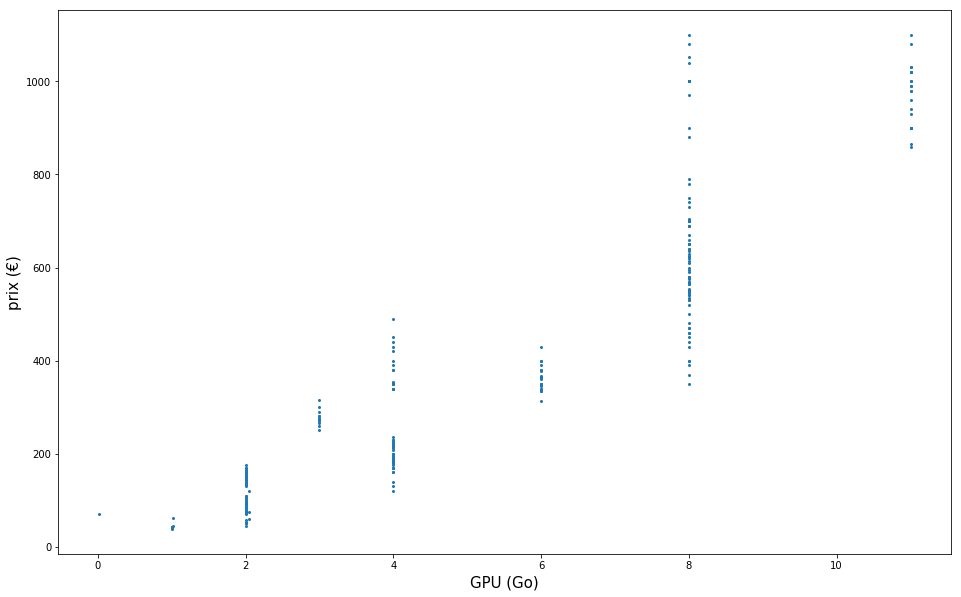
\includegraphics[width=0.8\textwidth]{figs/gpuPrices.png}    
  \end{figure}
\end{frame}

\begin{frame}{Construire un modèle (regression linéaire)}
  \begin{itemize}
  \item Soit: $x_{1}$ la valeur de GPU de nos $m$ carte graphiques, et $y$ leur prix
    \vspace{0.2cm}
  \item On cherche à déterminer le modèle pour prédire un prix $\hat{y}$ à partir $x_{1}$:
    \begin{equation*}
      \hat{y} = h_{\theta}(x_{1})
    \end{equation*}
  \item On défini le paramètre $\theta_{1}$ qui va \textit{lier} $x_{1}$ à $\hat{y}$:
    \begin{equation*}
      h_{\theta}(x) = \theta_{1} x_{1}
    \end{equation*}
  \item Rappel math: \textbf{fonction linéaire} $f(x) = kx$
  \end{itemize}
\end{frame}

\begin{frame}{Construire un modèle (regression linéaire)}
  \begin{itemize}
  \item Initialisons aléatoirement la valeur de $\theta_{1}$
  \end{itemize}
  \vspace{-0.5cm}
  \begin{figure}
    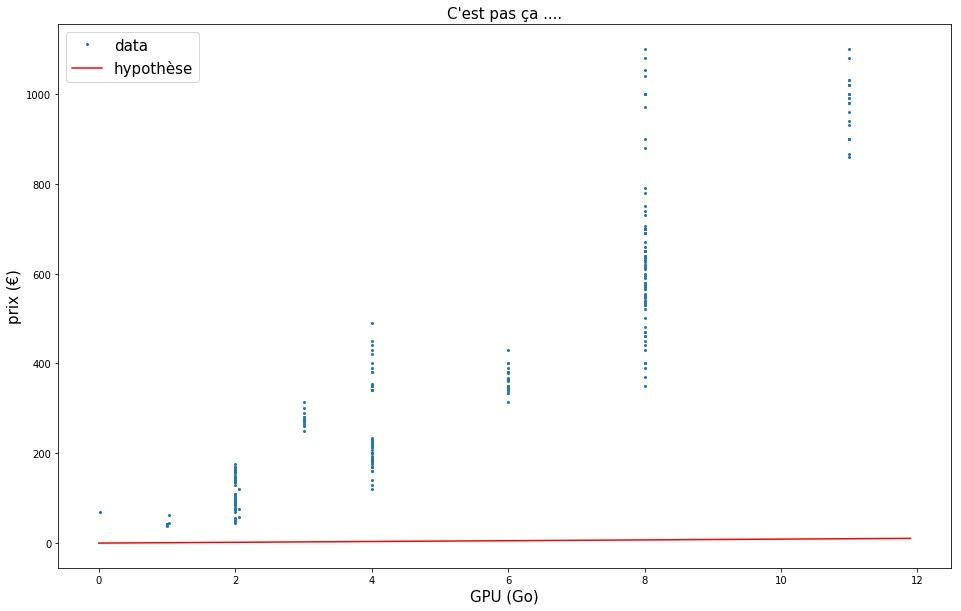
\includegraphics[width=0.8\textwidth]{figs/model.png}
  \end{figure}
  \vspace{-0.5cm}
  \begin{itemize}
  \item C'est pas encore ça ...
  \end{itemize}
\end{frame}

\begin{frame}{La fonction de coût}
  \begin{itemize}
  \item  $J(\theta)$: \textit{véracité} de notre modèle
  \item Une définition possible: somme quadratique des erreurs
      \begin{equation*}
        J(\theta) = \frac{1}{2m} \displaystyle\sum_{i=0}^{m}(\hat{y}^{(i)} - y^{(i)})^{2}
      \end{equation*}
  \end{itemize}
  \vspace{-0.5cm}
  \begin{figure}
    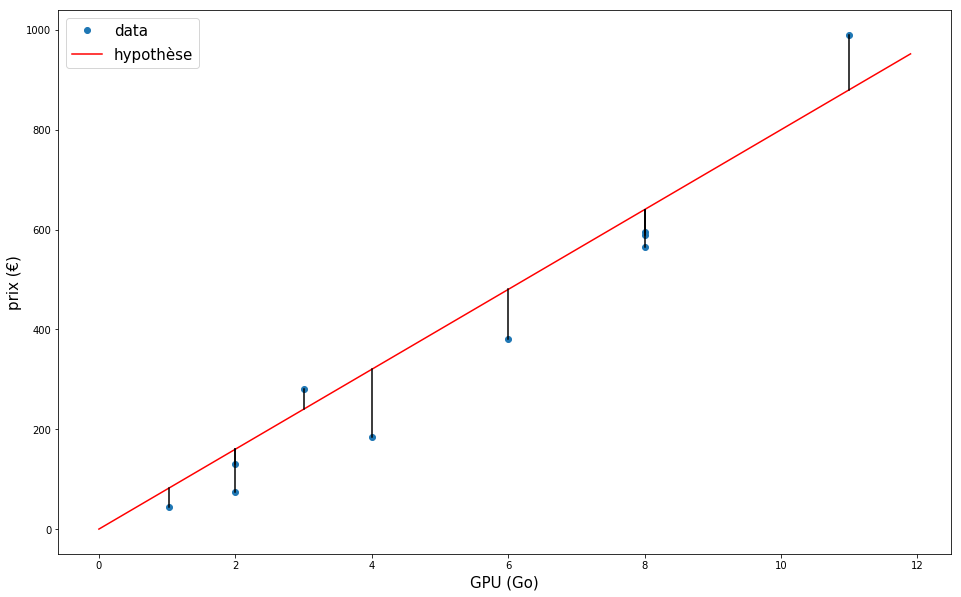
\includegraphics[width=0.8\textwidth]{figs/modelEstimation.png}
  \end{figure}  
\end{frame}

\begin{frame}{La fonction de coût}
  \begin{itemize}
  \item On cherche à trouver la valeur de $\theta_{1}$ qui \textbf{minimise} $J(\theta)$
    \vspace{0.2cm}
  \item En Brute ...
  \end{itemize}
  \vspace{-0.5cm}
  \begin{figure}
    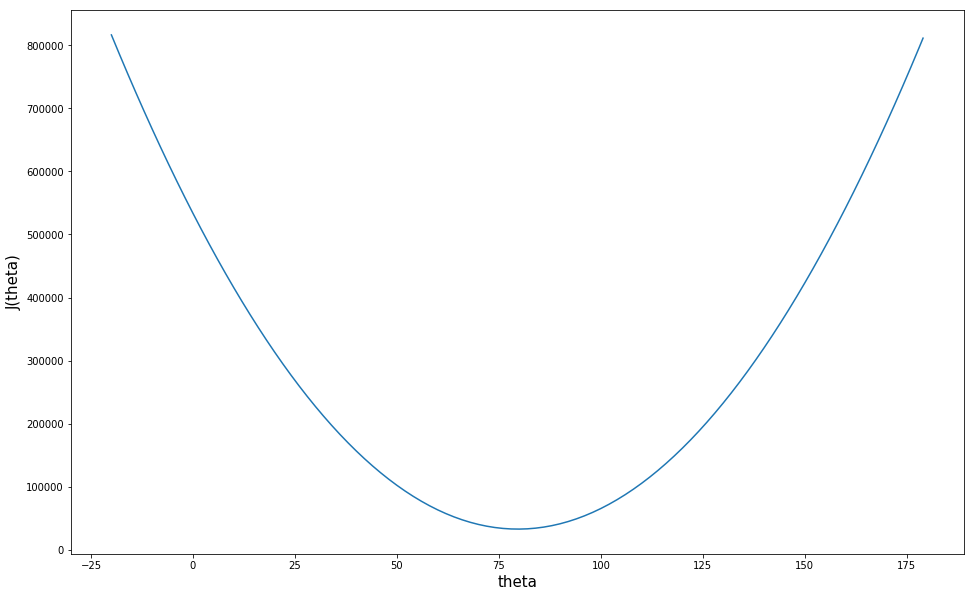
\includegraphics[width=0.8\textwidth]{figs/costFct.png}
  \end{figure}
  \vspace{-0.5cm}
  \begin{itemize}
  \item ... essayons d'optimiser
  \end{itemize}
\end{frame}

\begin{frame}{La descente de gradient}
  \begin{itemize}
  \item Algorithme pour arriver ``\textit{rapidement}'' au minimum de $J(\theta)$ 
    \vspace{0.2cm}
  \item On va utiliser la \textit{dérivation}: $\frac{d}{d\theta_{1}}J(\theta)$:
  \end{itemize}
  \begin{center}
    Si $J(\theta)$ est croissant: $\frac{d}{d\theta_{1}}J(\theta) > 0$, \hspace{0.5cm}
    Si $J(\theta)$ est décroissant: $\frac{d}{d\theta_{1}}J(\theta) < 0$
  \end{center}
  \vspace{-0.5cm}
  \begin{figure}
    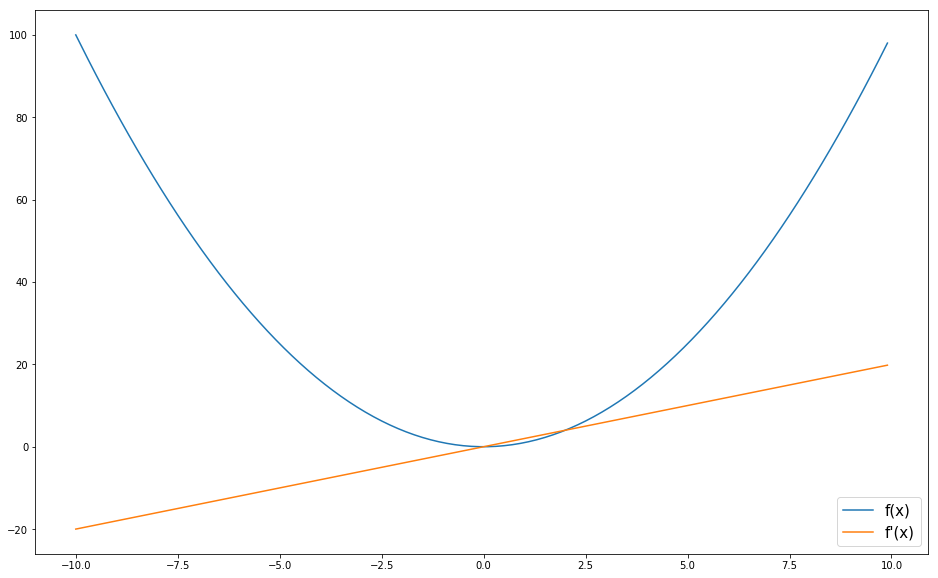
\includegraphics[width=0.7\textwidth]{figs/derivation.png}
  \end{figure}
  \vspace{-0.5cm}
\end{frame}

  
\begin{frame}{La descente de gradient}
  \begin{itemize}
  \item (Encore) un peu de math, la descente de gradient s'écrit:
  \end{itemize}
  \begin{beamerboxesrounded}[scheme=suppervise,width=\textwidth]{\textcolor{black}{Descente de gradient}}    
    \vspace{-0.2cm}
    \begin{equation*}
      \begin{matrix} \text{Répéter jusqu'à convergence:} & \{ & \\ & & \theta_{1} := \theta_{1} - \alpha \frac{d}{d\theta_{1}}J(\theta) \\ & \} & \end{matrix}
    \end{equation*}
    \vspace{-0.2cm}
    \end{beamerboxesrounded}
    \begin{itemize}
    \item $\alpha$ s'appelle le taux d'apprentissage (\textit{learning rate}) et c'est le \textbf{seul} paramètre de l'algorithme.
      \vspace{0.2cm}
    \item On va itérativement modifier la valeur de $\theta_{1}$ en fonction de la dérivée de $J(\theta)$, jusqu'à minimiser $J(\theta)$ (\textit{convergence}).
    \end{itemize}
\end{frame}

\begin{frame}{La descente de gradient}
  \begin{itemize}
  \item Dérivons donc notre fonction de coût:
  \end{itemize}
  \begin{equation*}
    J(\theta) = \frac{1}{2m} \displaystyle\sum_{i=0}^{m}(\hat{y}^{(i)} - y^{(i)})^{2} = \frac{1}{2m} \displaystyle\sum_{i=0}^{m}(\theta_{1}x_{1}^{(i)} - y^{(i)})^{2}
  \end{equation*}
  \begin{equation*}
      \frac{d}{d\theta_{1}}J(\theta) = \frac{1}{m}\displaystyle\sum_{i=0}^{m}(\hat{y}^{(i)} - y^{(i)}) x_{1}^{(i)}
  \end{equation*}
  \begin{itemize}
  \item Un peu de \textit{hand-tunning}:
    \begin{itemize}
      \normalsize
    \item Le learning rate ($\alpha$) est fixé à $0.03$ ($0.045$ pour la démo)
    \item Définissons une précision $\epsilon = 0.0001$ qui nous servira à arrêter la descente de gradient 
    \end{itemize}
  \end{itemize}
\end{frame}

\begin{frame}{Préparation du dataset}
  \begin{itemize}
  \item Bonne pratique de ML, pour tout les algos!
  \item On sépare \textbf{aléatoirement} les données en 2 (3) échantillons:
    \begin{itemize}
      \normalsize
    \item Entraînement / (Validation) / Test
    \item \textit{80 / 20} (\textit{70 / 30}) ou \textit{60 / 20 / 20}
    \end{itemize}
    \vspace{0.2cm}
  \item \textit{Entraînement:} utilisé pour la descente de gradient
  \item \textit{Validation:} utilisé pour l'hyperparamètrage de l'algo
  \item \textit{Test:} utilisé pour mesurer la performance du modèle
  \end{itemize}
\end{frame}

\begin{frame}{C'est parti !}
  \begin{figure}
    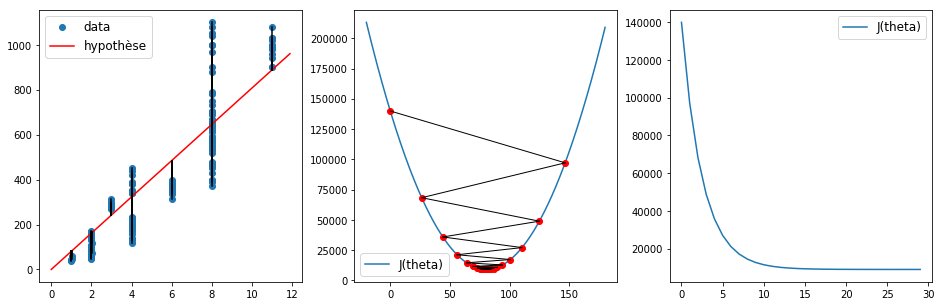
\includegraphics[width=\textwidth]{figs/gradDescent.png}
  \end{figure}
  \begin{itemize}
  \item La descente de gradient c'est achevée au bout de quelques itérations
  \item On peut voir que $J(\theta)$ a continuellement diminué à chaque itération
  \end{itemize}
  \begin{center}
    $\theta_{1} ~ \approx ~ 80$ \\
    $err_{train} ~ \approx ~ err_{test}$
  \end{center}
\end{frame}

\begin{frame}{On peut maintenant faire une prédiction}
  \begin{itemize}
  \item Quel serait le prix de cartes avec 5, 10 et 14 Go de GPU? 
  \end{itemize}
  \vspace{-0.2cm}
  \begin{figure}
    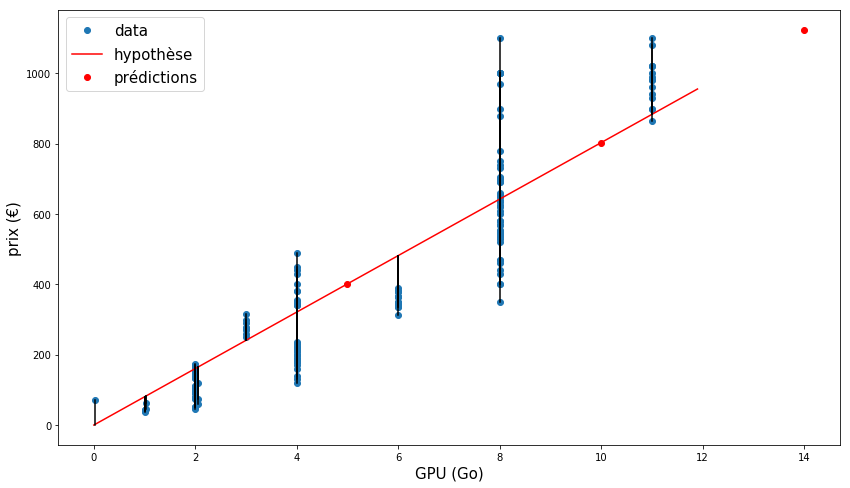
\includegraphics[width=0.8\textwidth]{figs/pred.png}
  \end{figure}
  \vspace{-0.5cm}
  \begin{itemize}
  \item On pourra les vendre autour de 400, 800 et 1100 euros!
  \end{itemize} 
\end{frame}

\begin{frame}{La regression linéaire multivariables}
  \begin{itemize}
    \item Le principe est le même, mais avec plusieurs variables $x_{i}$ (donc plusieurs paramètres $\theta_{i}$):
  \end{itemize}
    \begin{equation*}
      \hat{y} = \theta_{1}x_{1} + \dots + \theta_{n}x_{n} = \displaystyle\sum_{i=1}^{n} \theta_{i} x_{i}
    \end{equation*}
  \begin{figure}
    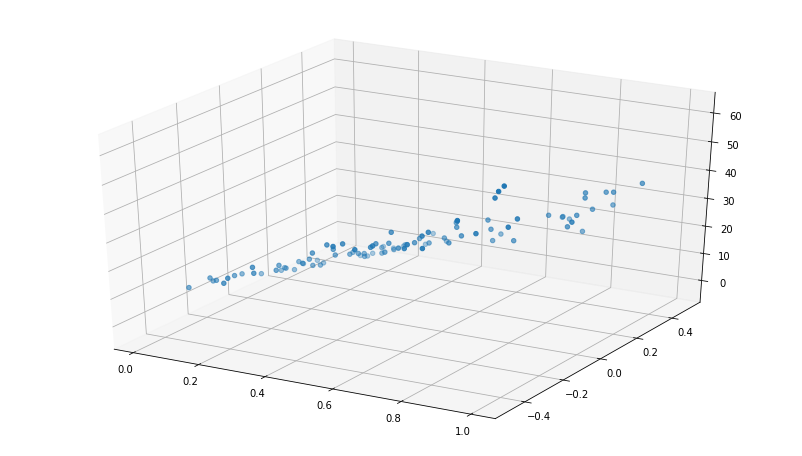
\includegraphics[width=0.45\textwidth]{figs/multiVarData.png}
    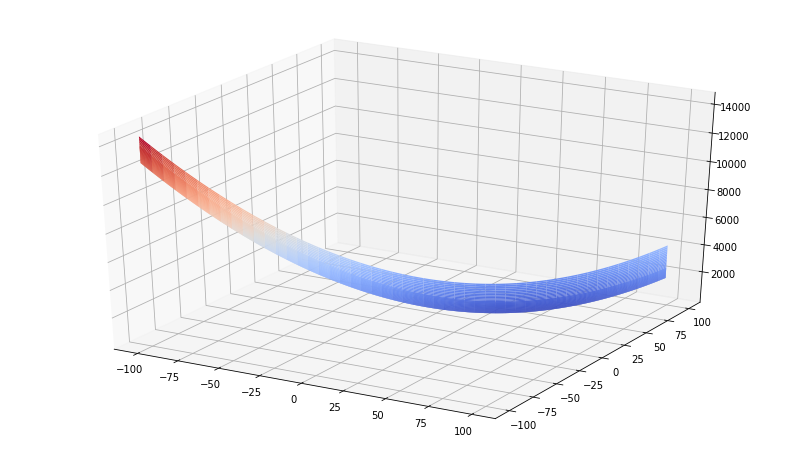
\includegraphics[width=0.45\textwidth]{figs/multiVarCostFct.png}\\
  \end{figure}
\end{frame}

\begin{frame}{Affinons notre modèle de carte graphiques}
  \begin{itemize}
  \item Plus de features: chipset, fréquence, consommation, ...
  \item Il va falloir explorer et nettoyer les données:
    \begin{itemize}
      \normalsize
    \item Gestion des données manquantes / abbérantes
    \item \textit{Features engineering}
    \item Normaliser le dataset (pour accélérer la descente de gradient)
    \end{itemize}
  \end{itemize}
\end{frame}

\begin{frame}{Régression linéaire multivariables: Résultats}
  \begin{itemize}
  \item On utilise la même valeur de $\epsilon = 0.0001$ et $\alpha = 0.03$
  \item Plus long! Mais meilleur résultats:
  \item Modèle simple: $err ~ \approx ~ 100$
  \item Modèle multivariable: $err ~ \approx ~ 30$
  \end{itemize}
  \begin{figure}
    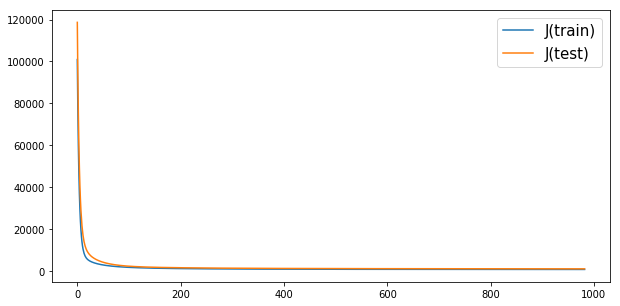
\includegraphics[width=0.45\textwidth]{figs/multiVarDesc.png}\\
  \end{figure}
\end{frame}
  
\begin{frame}{Pour conclure sur la régression linéaire}
  \begin{itemize}
  \item \textbf{Regression Linéaire:} $\hat{y}$ est une valeur \textit{continue}
    \begin{itemize}
    \item Valeur discrète: \textbf{Regression Logistique} (\textit{classification})
    \end{itemize}
    \vspace{0.2cm}
  \item Le résultat $\hat{y}$ dépend \textbf{linéairement} des variables $x_{i}$ si:
    \begin{equation*}
      \hat{y} = \theta_{1}x_{1} + \dots + \theta_{n}x_{n} = \displaystyle\sum_{i=1}^{n} \theta_{i} x_{i}
    \end{equation*}
  \item \textbf{Apprentissage supervisé}: $y$ est connu pour chaque $x_{1}$ dans le jeu de données d'entrainement
  \item Facile à implémenter (encore plus avec Scikit-learn ...), rapide: bon point de départ sur un sujet
  \end{itemize}
\end{frame}


\setbeamertemplate{background}{\pgfuseimage{bkg}}

\begin{frame}

  \vspace{5cm}
  \begin{center}
    \Large
    \textcolor{orange}{Merci !}\\
    \normalsize
    \vspace{0.5cm}
    Léo Beaucourt
  \end{center}

\end{frame}

\end{document}
